% !TeX root = ../main.tex

%\section{Model Formulation}

\subsection{Moving windows and the Short-time Fourier transform}
\label{subsec:STFT}

One issue with the CarHMM is that it assumes Markovian dynamics when conditioned on the hidden state, i.e. that any observation $Y^*_{t,t^*}$ depends only on the behavioral state $X^*_{t,t^*}$ and $Y^*_{t,t^*-1}$. However, there are many animal movement processes which violate this Markov property on very fine scales. For example, swimming behaviour of marine mammals is often exhibits periodic since the animal repeatedly flukes (swims up and down) to propel itself forward. Work has been done in the past to model non-Markovian dynamics in the \textit{behavioural} process $X^*_t$ \citep{Langrock:2012}, but to our knowledge addressing non-Markovian dynamics within the observation process $Y^*_t$ is still a relatively unstudied area \textcolor{red}{(MAYBE?)}. With improvements in tagging technology allowing for data to be collected at very high frequencies, noisy and non-Markovian fine scale behavior is likely to persist.

We borrow techniques from signal processing literature to compress the data and summarize its essential elements. In particular, we suggest performing the discrete-time short-time Fourier transform (STFT) over the observed fine-scale process $Y^*_t$:
%
\begin{align*}
    STFT\{Y^*_{t,(s^*h+1):(s^*h+h) }\}(k) := \hat{Y}^{*(k)}_{t,s^*} = \sum_{n = 1}^{h} Y^*_{t,(s^*h)+n}e^{-i \frac{2\pi k}{h} (n-1)} \\ k = 0, 1, \ldots, h-1; \quad s^* = 0,1, \ldots, \lfloor T^*_t / h \rfloor - 1
\end{align*}
%
Where $i$ in the equation above refers the $\sqrt{-1}$. The STFT slides a moving window of length $h$ across the time series $Y_t^*$ and transforms the domain of each window from time to frequency. This allows the spectrum of $Y_t^*$ at time $t^*$ to be summarized by a $h$-dimensional vector of Fourier coefficients. While other step sizes can be used for the sliding window, we select $h$ to avoid serial dependence between windows. Note here that $s^*$ indexes the \textit{windows} moving across $Y^*_t$ while $t^*$ indexes the \textit{observations} of $Y^*_t$. 

If $Y^*_t \in \mathbb{R}^{T^*_t}$, then $\hat{Y}_t^* \in \mathbb{C}^{\lfloor T^*_t / h \rfloor \times h}$. Although this allows $Y^*_t$ to be represented in a way that eliminates obvious periodic behavior, the data set itself is still approximately as large as $Y^*_t$ itself. To reduce the size of $\hat{Y}^*_t$, we take two summary statistics of each window:
%
$$Z_{t,s^*}^{*(1)} = \mathcal{R}\left(\hat{Y}^{*(0)}_{t,s^*}\right) \qquad Z_{t,s^*}^{*(2)} = \frac{1}{h}\sum_{k=1}^{\tilde{f}}|\hat{Y}^{*(k)}_{t,s^*}|^2$$
%
$Z_{t,s^*}^{*(1)}$ is equal to the average value of $Y_{t,s^*}^*$, and $Z_{t,s^*}^{*(2)}$ is equal to the squared 2-norm of the component of $Y_{t,s^*}^*$ that can be attributed to frequencies in the signal between $1$ and $\tilde{f}$ periods per window length. Both the window length $h$ and the max frequency $\tilde{f}$ are problem-specific tuning parameters. $h$ should be long enough to capture the periodic behavior of the underlying process (at least as long as the length of a period), but short enough to avoid over-smoothing of the data and to maintain high resolution in the behavioral process $X^*$. $\tilde{f}$ should be selected such that $\tilde{f}$ periods per window length is the maximum frequency of $Y_t^*$ that makes biological sense. Note that these summary statistics are just one possible choice to describe each window, and other choices include the maximum and argmax of $\hat Y^*_{t,s^*}$. Future studies can adjust these definitions as needed. A visualization of transforming a one-dimensional sequence $Y^*$ to $Z^*$ can be seen in figure (\ref{fig:fourier_example}).

\begin{figure}[ht]
	\centering
	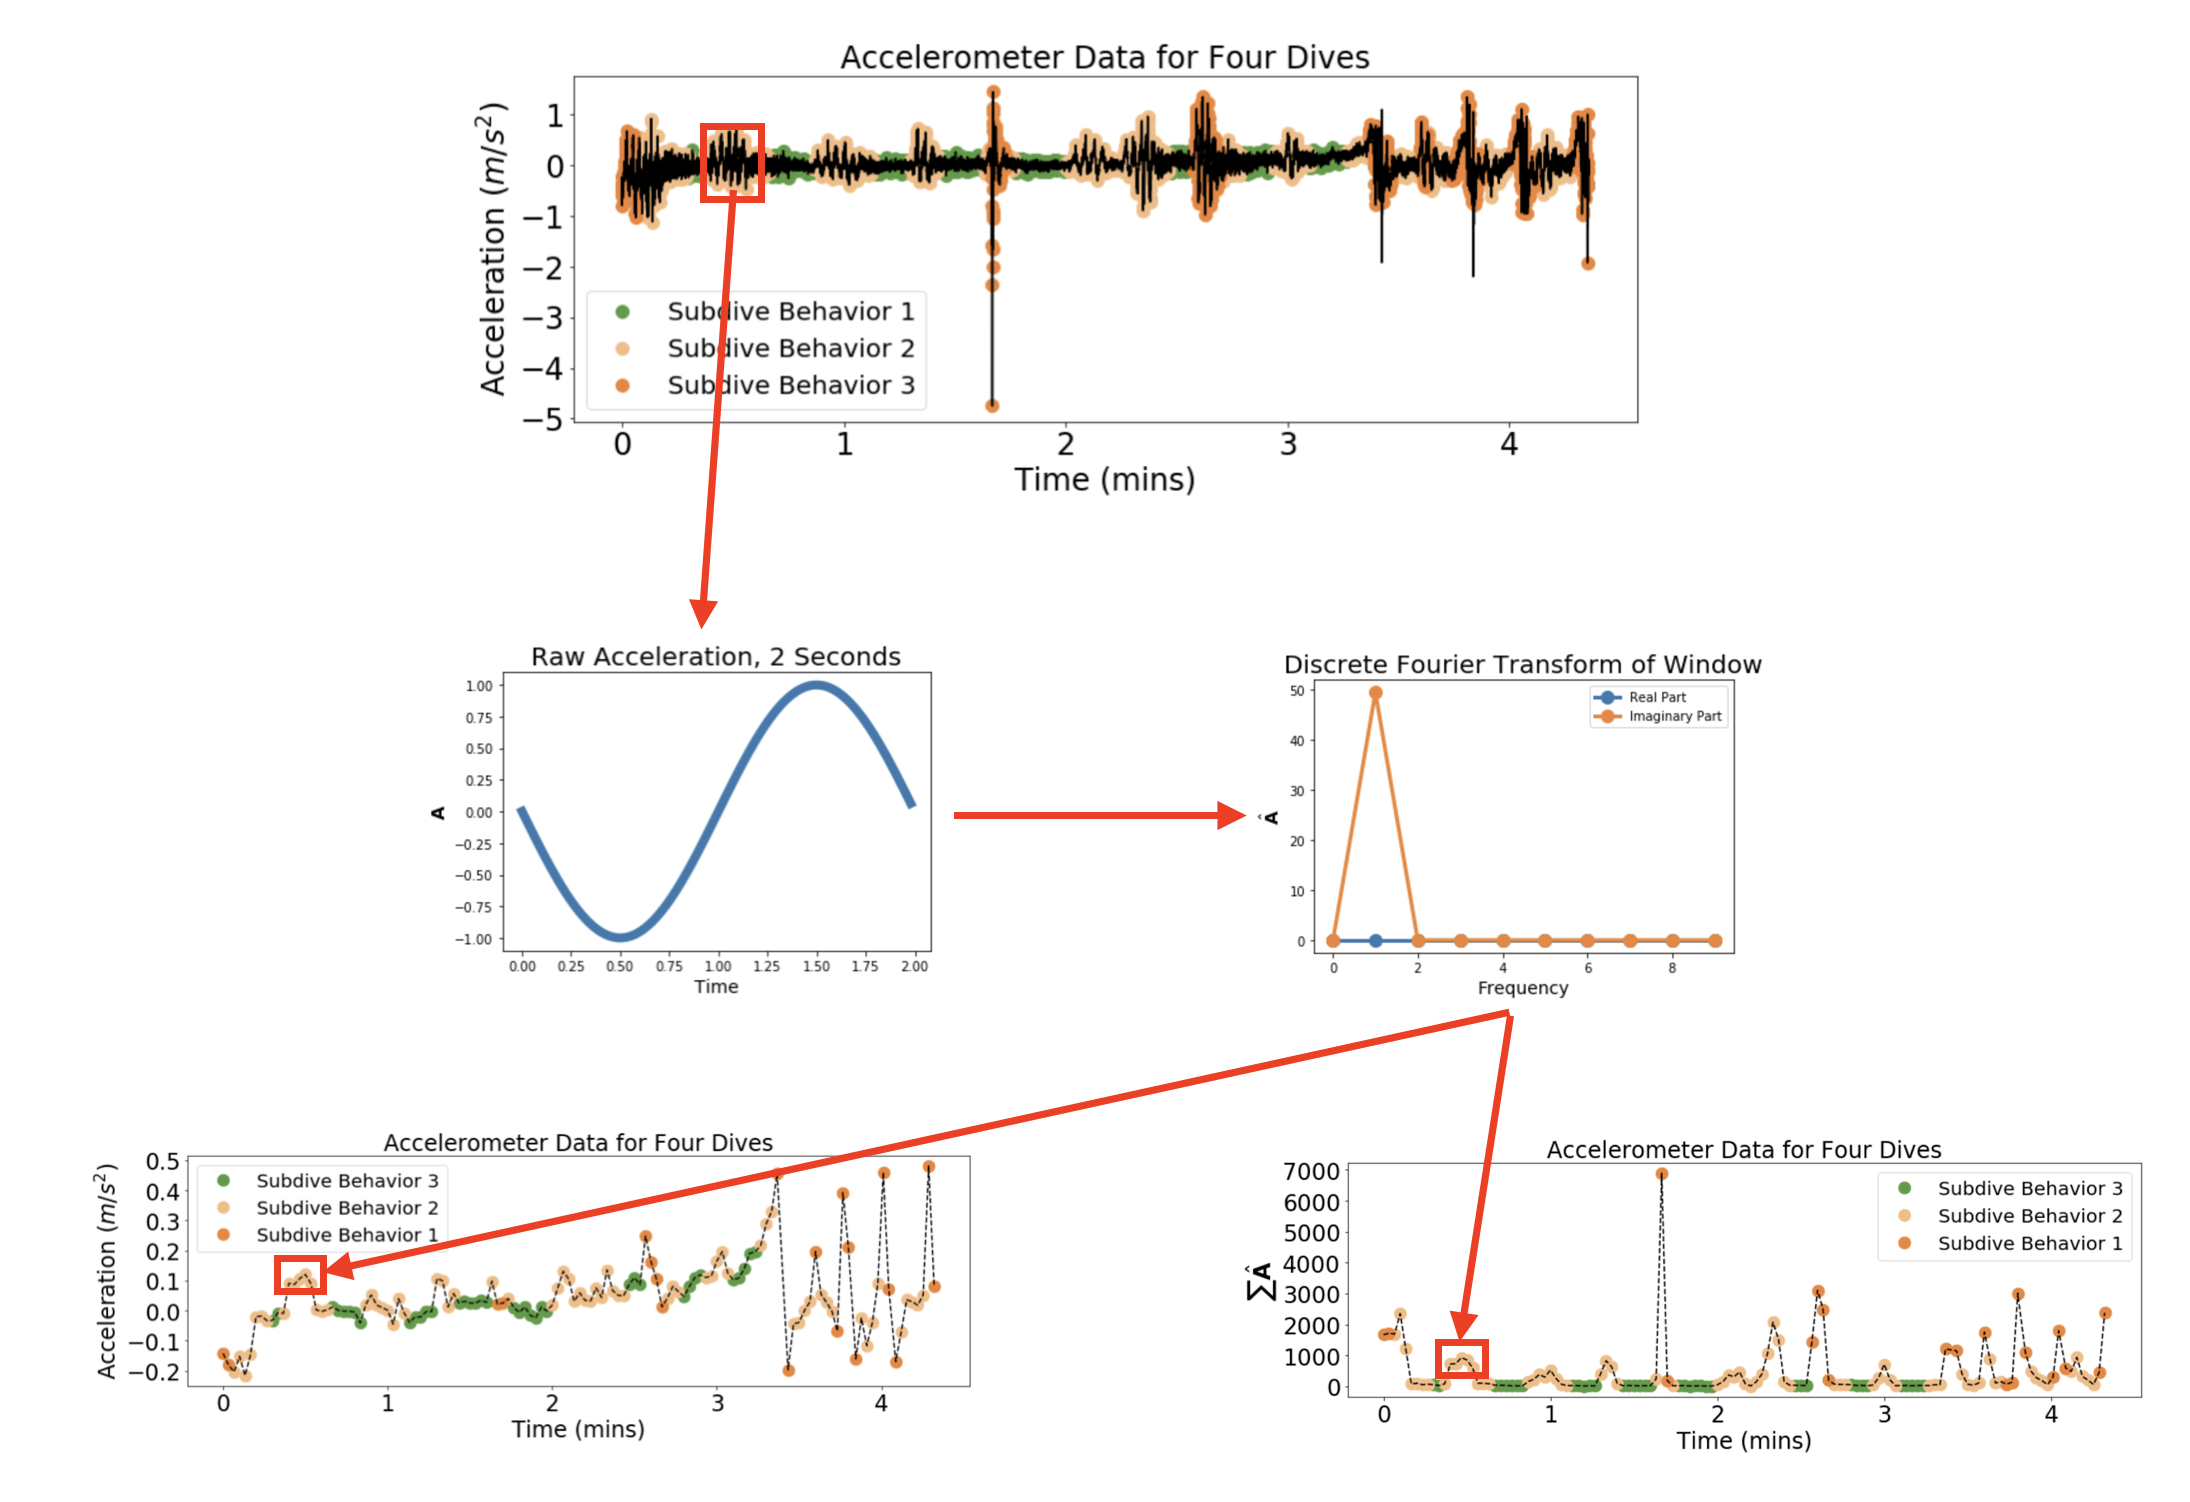
\includegraphics[width=5in]{../Plots/fourier_transform.png}
	\caption{Visualization of transforming $Y^*_t$ into $Z^*_t$ using a sliding window and Fourier transform.}
	\label{fig:fourier_example}
\end{figure}

It is possible to accommodate for unequal time steps within each window by using the \textbf{non-uniform discrete Fourier transform (NDFT)}. We do not describe the details of this method in this work, but the generalization is straightforward. Refer to Bagchi et al \citep{Bagchi:1999} for details.

The advantages of using Fourier analysis within an HMM has been recently demonstrated in the context of describing daily behavioral cycles of marine mammals \citep{Heerah:2017}. In addition, Fourier analysis has previously been used in the field of animal movement to explain animal behavior \citep{Fehlmann:2017} and specifically fluking \citep{Shorter:2017} from accelerometer data. Thus, incorporating Fourier analysis of accelerometer data within the structure of an HMM appeared a promising simple approach to account for additional correlation in data that is cyclical in nature.

\subsection{Model Structure: combining the HHMM and CarHMM}
\label{subsec:model_structure}

Hierarchical hidden Markov models can be used to jointly model simultaneous coarse-scale and fine-scale processes. However, as mentioned before, the fine-scale process $Y^*$ can often exhibit auto-correlation and intricate structure. Transforming $Y^*_t$ to $Z^*_t$ removes fine-scale periodic behavior, but $Z^*_t$ can still exhibit auto-correlation, especially in $Z_{t,s^*}^{*(1)}$. Therefore, we replace the fine-scale HMM within the hierarchical HMM with a CarHMM as shown in (fig \ref{fig:CarHHMM}).
%
\begin{figure}[ht]
	\centering
	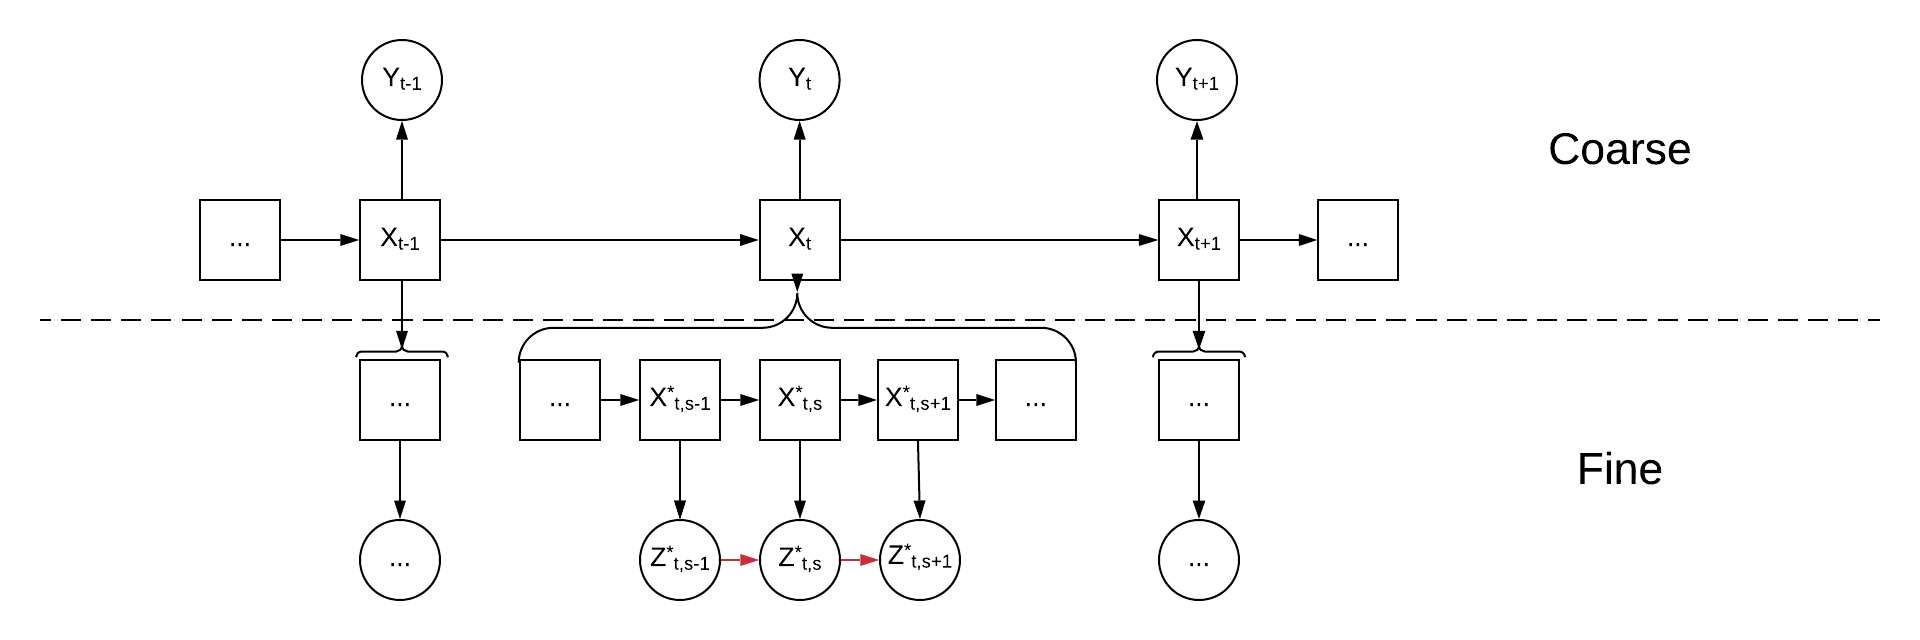
\includegraphics[width=5in]{../Plots/CarHHMM.png}
	\caption{Graphical representation of a CarHHMM. The additional arrows representing auto-correlation between observations are shown in red for emphasis.}
	\label{fig:CarHHMM}
\end{figure}
%
Naturally, we refer to this model as the \textbf{CarHHMM}, and it can be implemented both with and without the short-time Fourier-transform (STFT). The likelihood of this model is still easy to calculate using the forward algorithm:
%
$$\calL_{\text{CarHHMM}}(y,z^*;\Theta,\Theta^*,\Gamma,\Gamma^*) = \delta P(y_1,z_1^*;\Theta,\Theta^*,\Gamma^*) \prod_{t=2}^T \Gamma P(y_t,z_t^*;\Theta,\Theta^*,\Gamma^*) \mathbf{1}_N$$
%
where:
%
\begin{align*}
P(y_t,z_t^*;\Theta,\Theta^*,\Gamma^*)  = \text{diag}\Big[&f^{(1)}(y_t)\calL_{\text{CarHMM}}\left(z_t^*;\Theta^{*(1)},\Gamma^{*(1)}\right), \ldots , \\
&f^{(N)}(y_t)\calL_{\text{CarHMM}}\left(z_t^*;\Theta^{*(N)},\Gamma^{*(N)}\right) \Big]
\end{align*}
%